%%% ======= Beamer ======
\documentclass[usenames,dvipsnames,t]{beamer}
% \documentclass[usenames,dvipsnames, handout]{beamer}
\beamertemplatenavigationsymbolsempty % remove toolbar at the bottom of slides
\usepackage{appendixnumberbeamer} % for appendix
\usetheme{Madrid}
\usecolortheme{default}
\useinnertheme{circles}

\setbeamercolor{author in head/foot}{bg=blue!10, fg=blue}
\setbeamercolor{title in head/foot}{bg=blue!10, fg=blue}
\setbeamercolor{date in head/foot}{bg=blue!10, fg=blue}

\makeatletter
\setbeamertemplate{footline}{
  \leavevmode%
  \hbox{%
  \begin{beamercolorbox}[wd=.333333\paperwidth,ht=2.25ex,dp=1ex,center]{author in head/foot}%
    \usebeamerfont{author in head/foot}\insertshortauthor\expandafter\ifblank\expandafter{\beamer@shortinstitute}{}{~~(\insertshortinstitute)}
  \end{beamercolorbox}%
  \begin{beamercolorbox}[wd=.333333\paperwidth,ht=2.25ex,dp=1ex,center]{title in head/foot}%
    \usebeamerfont{title in head/foot}\insertshorttitle
  \end{beamercolorbox}%
  \begin{beamercolorbox}[wd=.333333\paperwidth,ht=2.25ex,dp=1ex,right]{date in head/foot}%
    \usebeamerfont{date in head/foot}\insertshortdate{}\hspace*{2em}
    \insertframenumber{}%
%     / \inserttotalframenumber
    \hspace*{2ex} 
  \end{beamercolorbox}}%
  \vskip0pt%
}
\makeatother

\colorlet{beamer@blendedblue}{blue!70} % change color theme


% For appendix
\newcommand{\backupbegin}{
   \newcounter{framenumberappendix}
   \setcounter{framenumberappendix}{\value{framenumber}}
}
\newcommand{\backupend}{
   \addtocounter{framenumberappendix}{-\value{framenumber}}
   \addtocounter{framenumber}{\value{framenumberappendix}} 
}

\setbeamertemplate{bibliography item}{\insertbiblabel} % improved references



% Other preamble stuff:
\usepackage{preamble}

%%% Uncomment for another color palette
% \definecolor{Logo1}{rgb}{0.0, 0, 0.7}
% \definecolor{Logo2}{rgb}{2.55, 2.55, 2.55}

% \setbeamercolor*{palette primary}{bg=Logo1, fg=white}
% \setbeamercolor*{palette secondary}{bg=Logo2, fg=white}
% \setbeamercolor*{palette tertiary}{bg=white, fg=Logo1}
% \setbeamercolor*{palette quaternary}{bg=white,fg=white}
% \setbeamercolor{structure}{fg=Logo1} % itemize, enumerate, etc
% \setbeamercolor{section in toc}{fg=Logo1} % TOC sections

% For figures
\usepackage{import}
\usepackage{xifthen}
\usepackage{pdfpages}
\usepackage{transparent}
\usepackage{mdframed}

% --- Inkscape figures:
\newcommand{\incfig}[2][0.75\textwidth]{%
    \def\svgwidth{\columnwidth}
    \resizebox{#1}{!}{\import{Inkscape figs/}{#2.pdf_tex}}
}

% --- Height of frame
\newlength{\myheight}
\setlength{\myheight}{7cm}


%------------------------------------------------------------
%This block of code defines the information to appear in the
%Title page
\title[QCD JC] %optional
{Current and future prospects on EOS constraints from gravitational waves}

\author{Thibeau Wouters}

\date{January 30, 2024}




%End of title page configuration block
%------------------------------------------------------------



%------------------------------------------------------------
%The next block of commands puts the table of contents at the 
%beginning of each section and highlights the current section:

\AtBeginSection[]
{
  \begin{frame}[plain, noframenumbering]
    \frametitle{Table of Contents}
    \tableofcontents[currentsection]
  \end{frame}
}

\AtBeginSubsection[]
{
  \begin{frame}[plain, noframenumbering]
    \frametitle{Table of Contents}
    \tableofcontents[currentsection]
  \end{frame}
}


%------------------------------------------------------------


\begin{document}

{

\usebackgroundtemplate{\transparent{0.30}{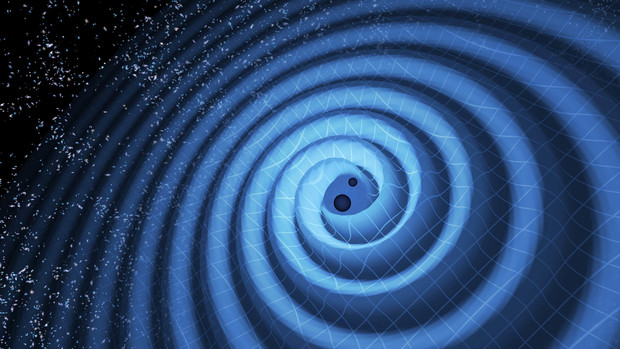
\includegraphics[width=\paperwidth,height=\paperheight]{Figures/GW-2.jpeg}}}


\begin{frame}[plain]
\titlepage

% \begin{figure}
% \centering
% 
\includegraphics[width=0.25\textwidth]{Figures/utrecht-university.png}
% \end{figure}

\end{frame}
}

% %The next statement creates the title page.
% \frame[plain]{\titlepage



% }


%---------------------------------------------------------
%This block of code is for the table of contents after
%the title page
\begin{frame}[plain, noframenumbering]
\frametitle{Table of Contents}
\tableofcontents
\end{frame}
%---------------------------------------------------------


\section{Introduction}

\begin{frame}{Gravitational waves}

  \def\x{3mm}

\begin{itemize}
  \item So far: compact binary coalescences (CBC) observed, black holes and neutron stars
  
  \vspace{\x}

  \item Measure \red{strain} $h(t) = \delta L(t) / L$ (\href{https://www.youtube.com/watch?v=UA1qG7Fjc2A}{animation})
  
  \vspace{\x}

  \item 3 phases: inspiral, merger, ringdown
\end{itemize}

\begin{figure}[H]
  \centering
  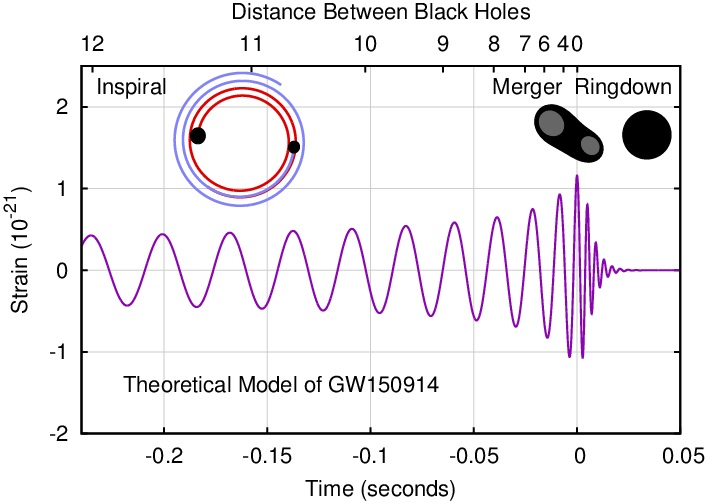
\includegraphics[width=0.5\textwidth]{Figures/GW150914.jpeg}
\end{figure}
\end{frame}

\begin{frame}{Gravitational wave detectors}

  \begin{itemize}
    \item Currently: LIGO (Hanford, Livingston), Virgo (Italy), KAGRA (Japan)
  \end{itemize}

  \begin{columns}
    
    \column{0.45\textwidth}
    \begin{figure}[H]
      \centering
      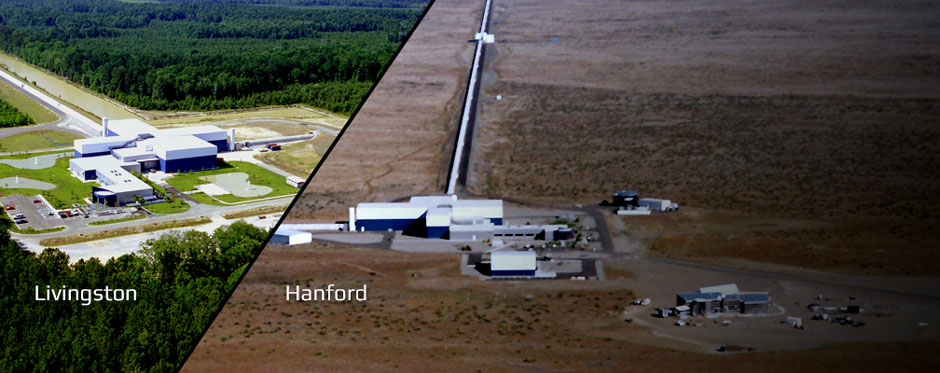
\includegraphics[width=0.75\textwidth]{Figures/ifo-Livingston-Hanford.jpeg}
    \end{figure}

    \column{0.45\textwidth}
    \begin{figure}[H]
      \centering
      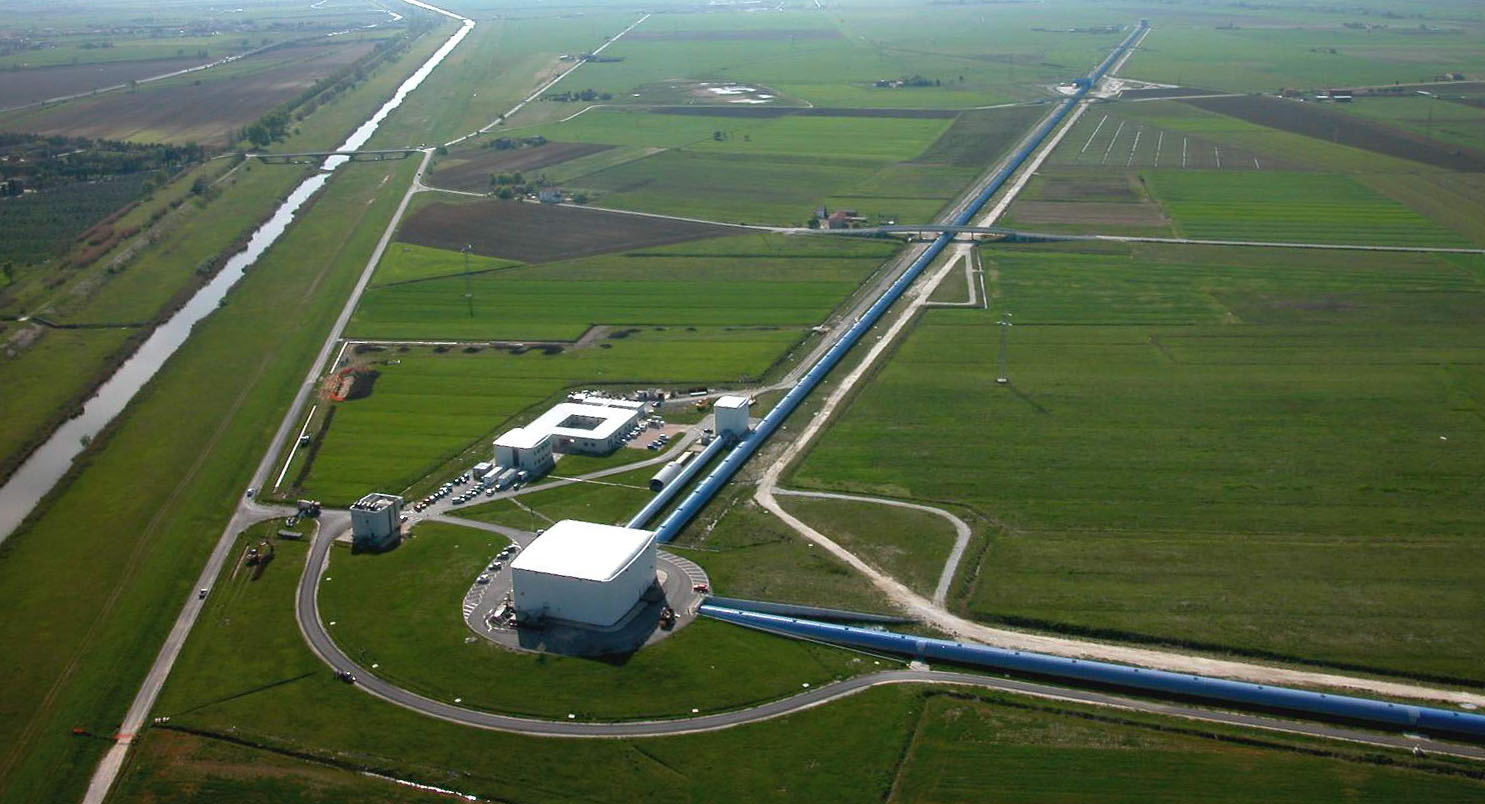
\includegraphics[width=0.75\textwidth]{Figures/Virgo.jpeg}
    \end{figure}
  \end{columns}

  \begin{itemize}
    \item Future: Einstein Telescope (ET), Cosmic Explorer (CE), LISA, ...
  \end{itemize}
  \begin{figure}
    \centering
    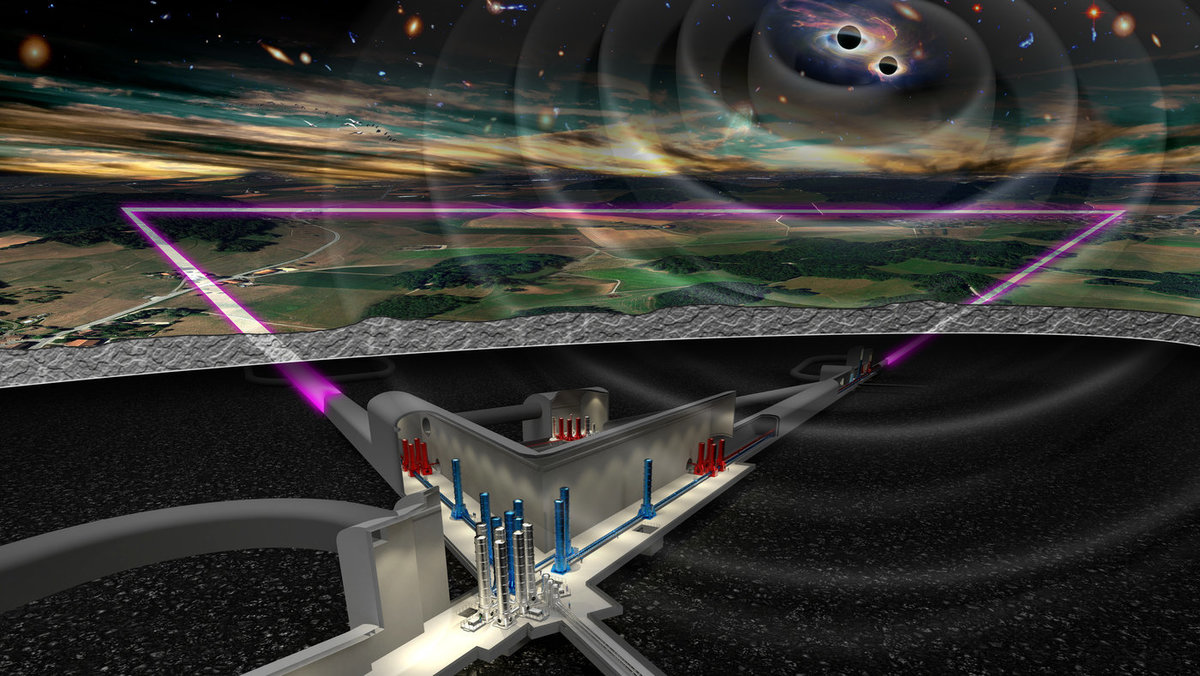
\includegraphics[width=0.5\textwidth]{Figures/einstein-telescope.jpeg}
  \end{figure}
  
\end{frame}

\section{Current methods \& results}

\begin{frame}{Tidal deformability}

  \def\x{3mm}

  \begin{itemize}
    \item Extended objects (neutron stars): tidally deformed in presence of external gravitational field $\mathcal{E}_{ij}$
    
    \vspace{\x}

    \item Develop quadrupole moment: $Q_{ij} = - \lambda \mathcal{E}_{ij}$, $\red{\lambda} =$ tidal deformability
    
    \vspace{\x}

    \item Modifies \textbf{inspiral} phase of GW: 
    \begin{align*}
      \tilde{h}(f) &= A \exp{i \Psi(f)} \\ 
      \Psi(f) &= \Psi_{\text{point}}(f) + \blue{\Psi_{\text{tidal}}(f)(\Lambda_1, \Lambda_2)} \, .
    \end{align*}

  \end{itemize}

  \begin{figure}[H]
    \centering
    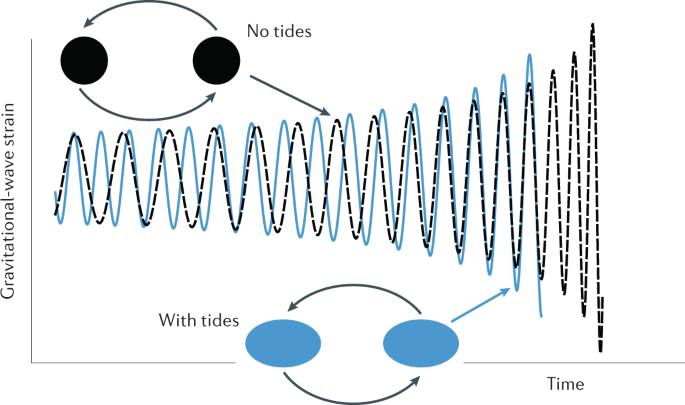
\includegraphics[width=0.5\textwidth]{Figures/tidal-deformations.png}
  \end{figure}
\end{frame}

  
\begin{frame}{Relation with EOS}
  
  The tidal deformability is linked to the EOS: a $(P, \rho)$ curve maps to a $(M, \Lambda)$ curve.
  
  \begin{columns}
    \column{0.45\textwidth}
    \begin{figure}[H]
      \centering
      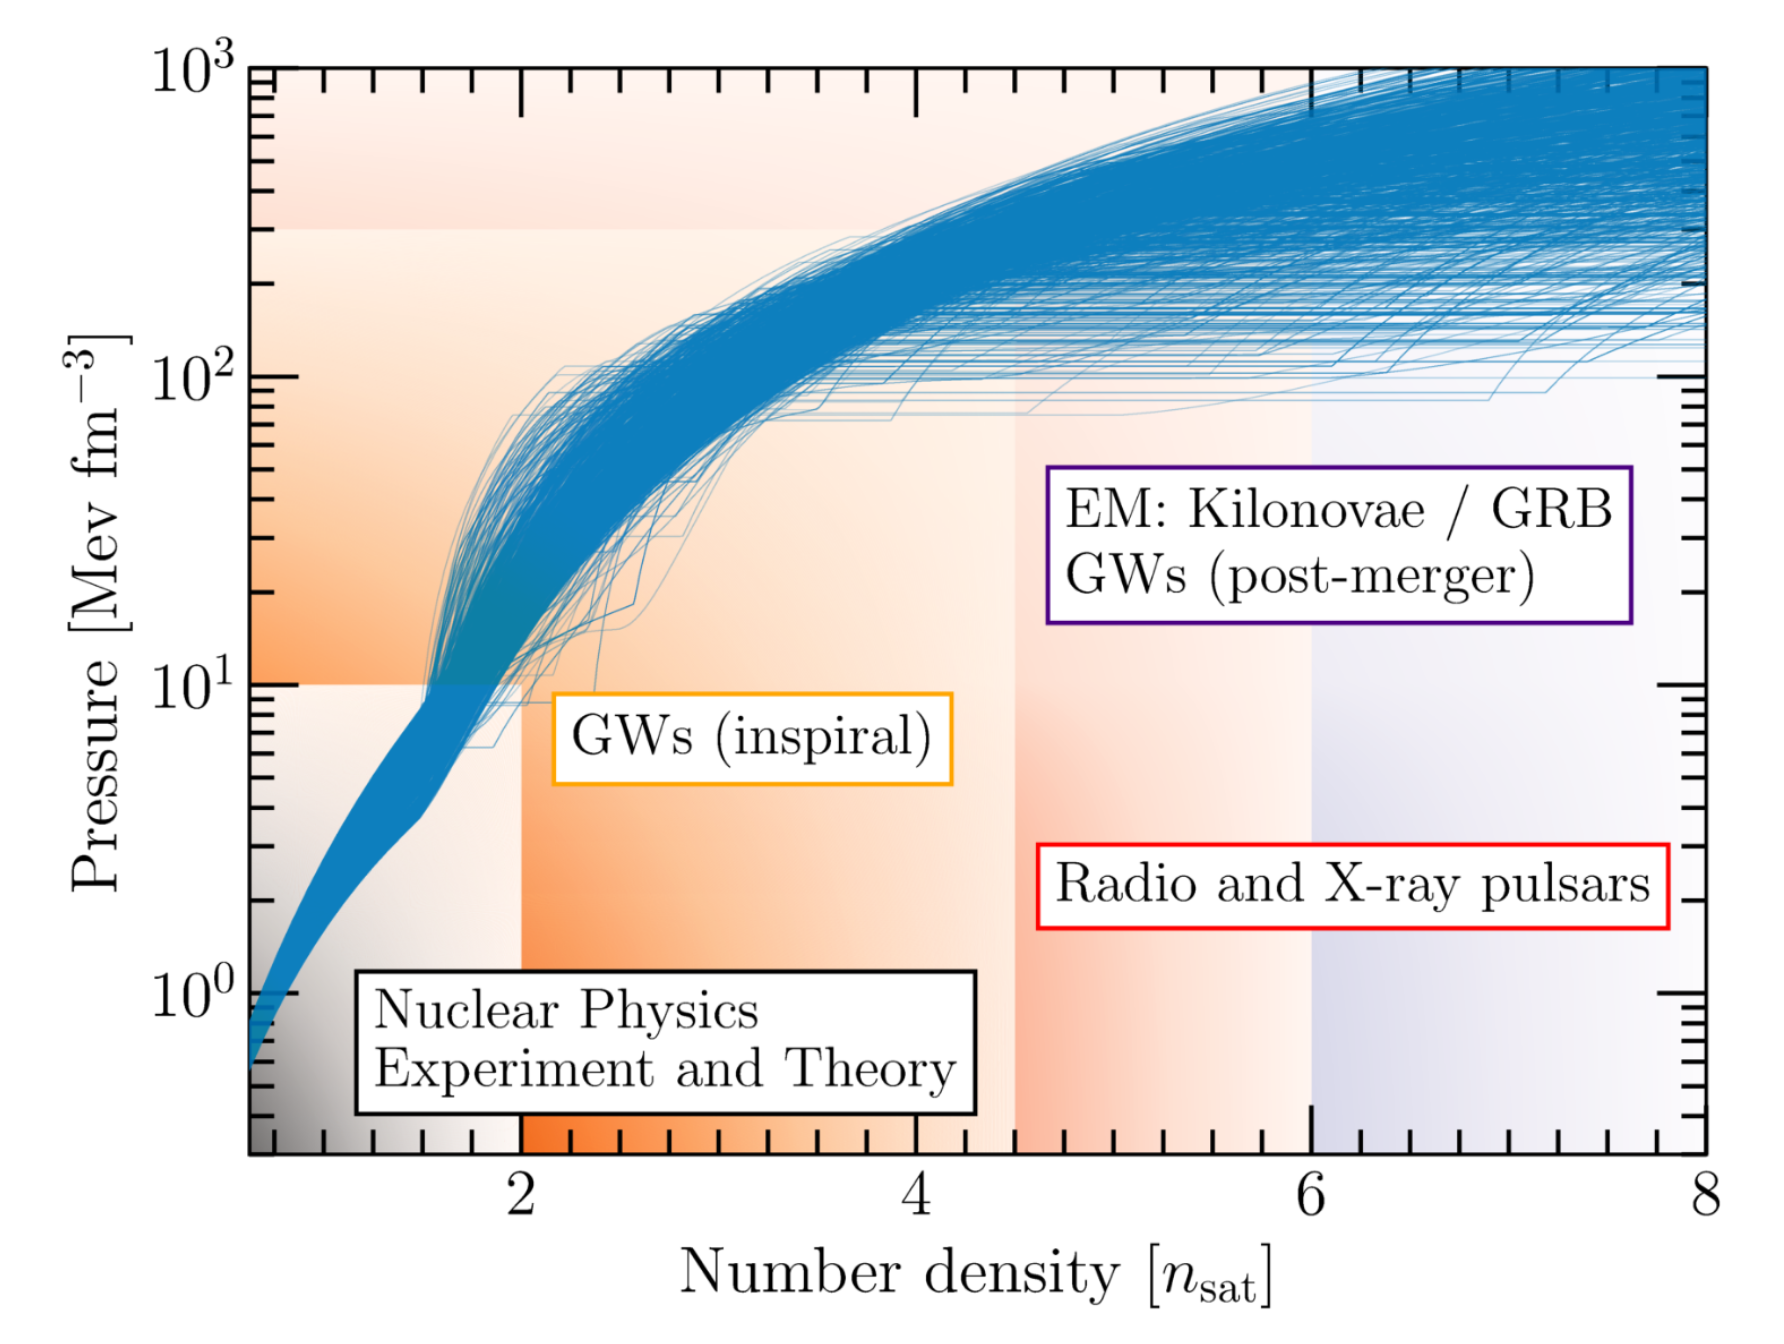
\includegraphics[width=\textwidth]{Figures/EOS-PV.png}
    \end{figure}

    \column{0.45\textwidth}
    \begin{figure}[H]
      \centering
      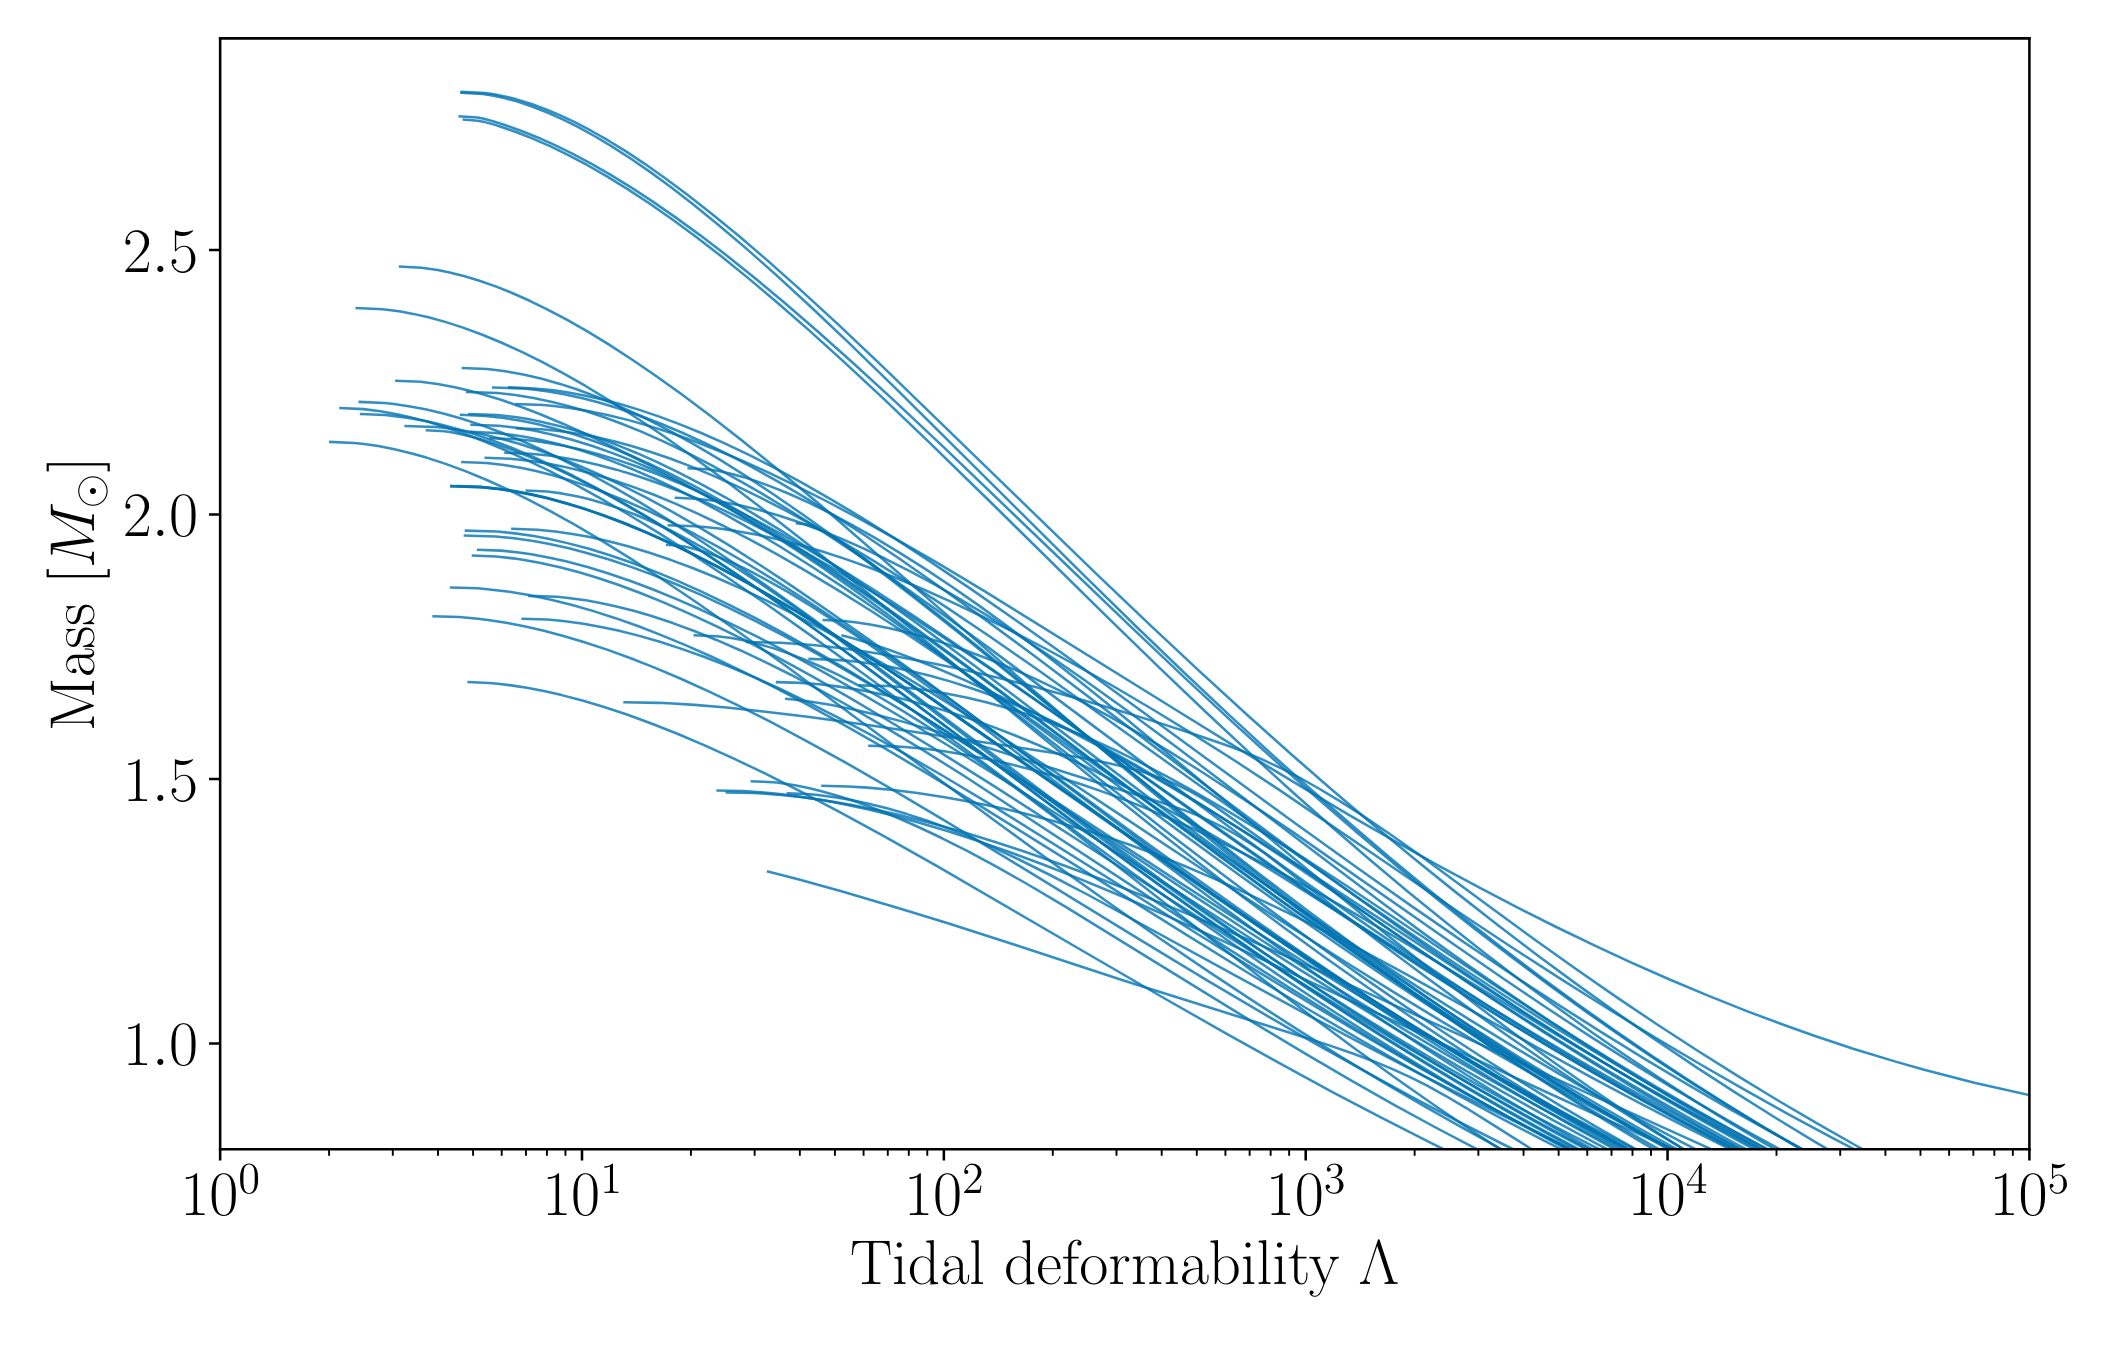
\includegraphics[width=\textwidth]{Figures/EOS-ML.png}
    \end{figure}
  \end{columns}

  \begin{tcolorbox}[colback=blue!5,colframe=blue!75!black]
    Inspiral of neutron stars $\rightarrow$ measure $(M, \Lambda)$ $\rightarrow$ constrain EOS
  \end{tcolorbox}

\end{frame}


\begin{frame}{Results}

  \def\x{3mm}

  GW170817: first binary neutron star merger observed~\cite{GW170817_properties}.
  
  \only<2>{
    \begin{equation*}
      \tilde{\Lambda} = \frac{16}{13} \frac{(m_1 + 12 m_2) m_1^4 \Lambda_1 + (m_2 + 12 m_1) m_2^4 \Lambda_2}{(m_1 + m_2)^5} \, .
    \end{equation*}
  }

  \only<1>
  {
    \begin{figure}
      \centering
      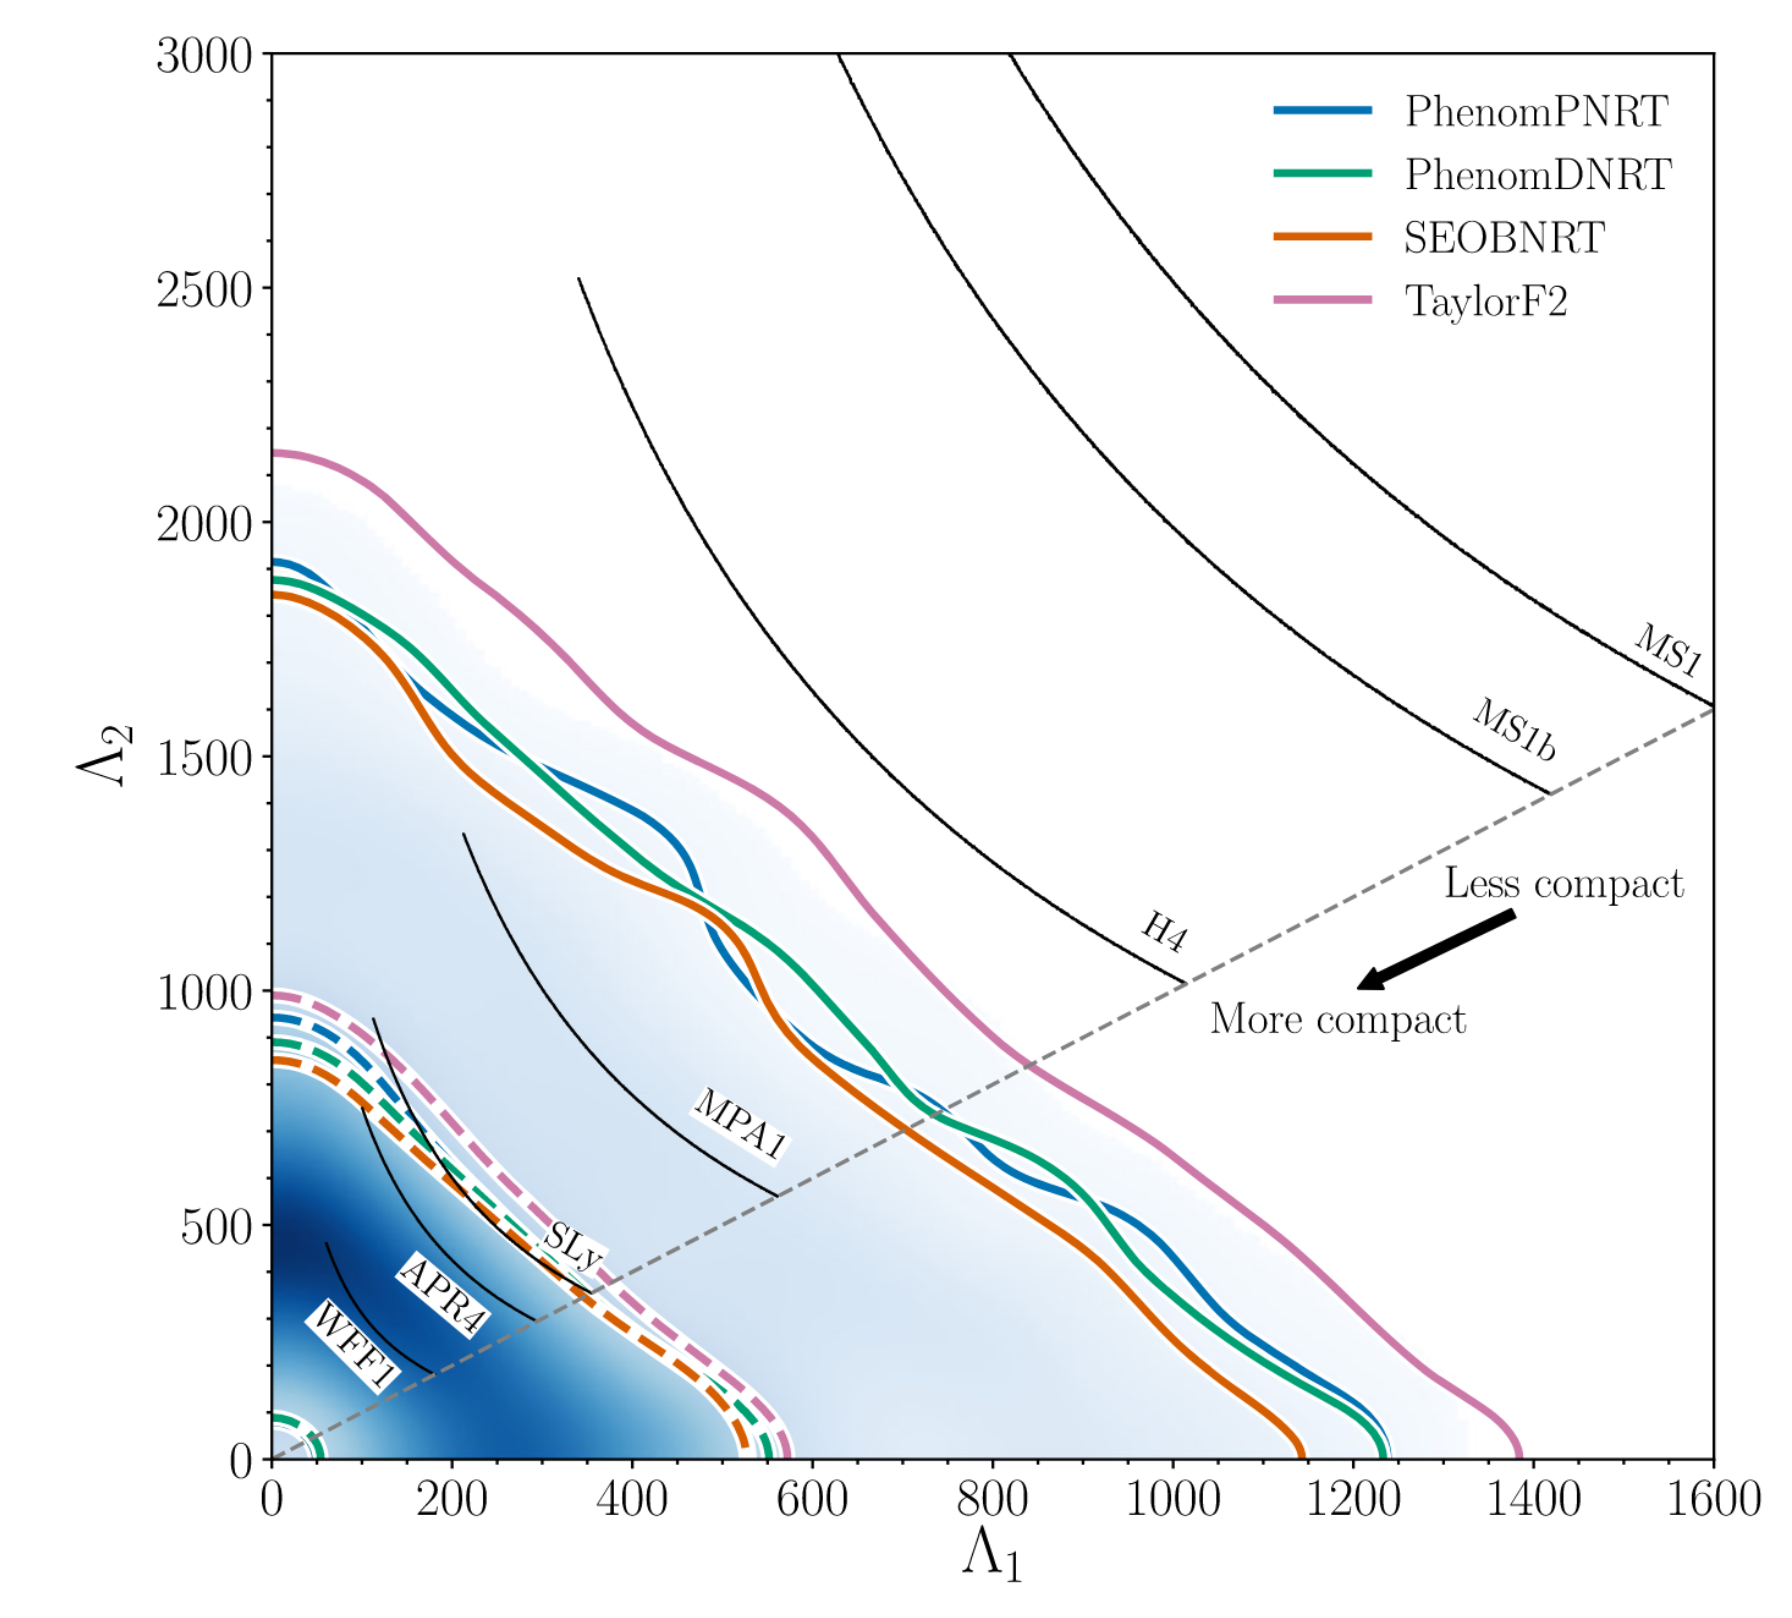
\includegraphics[width=0.6\textwidth]{Figures/GW170817_lambdas.png}
    \end{figure}
  }

  \only<2>
  {
    \begin{figure}
      \centering
      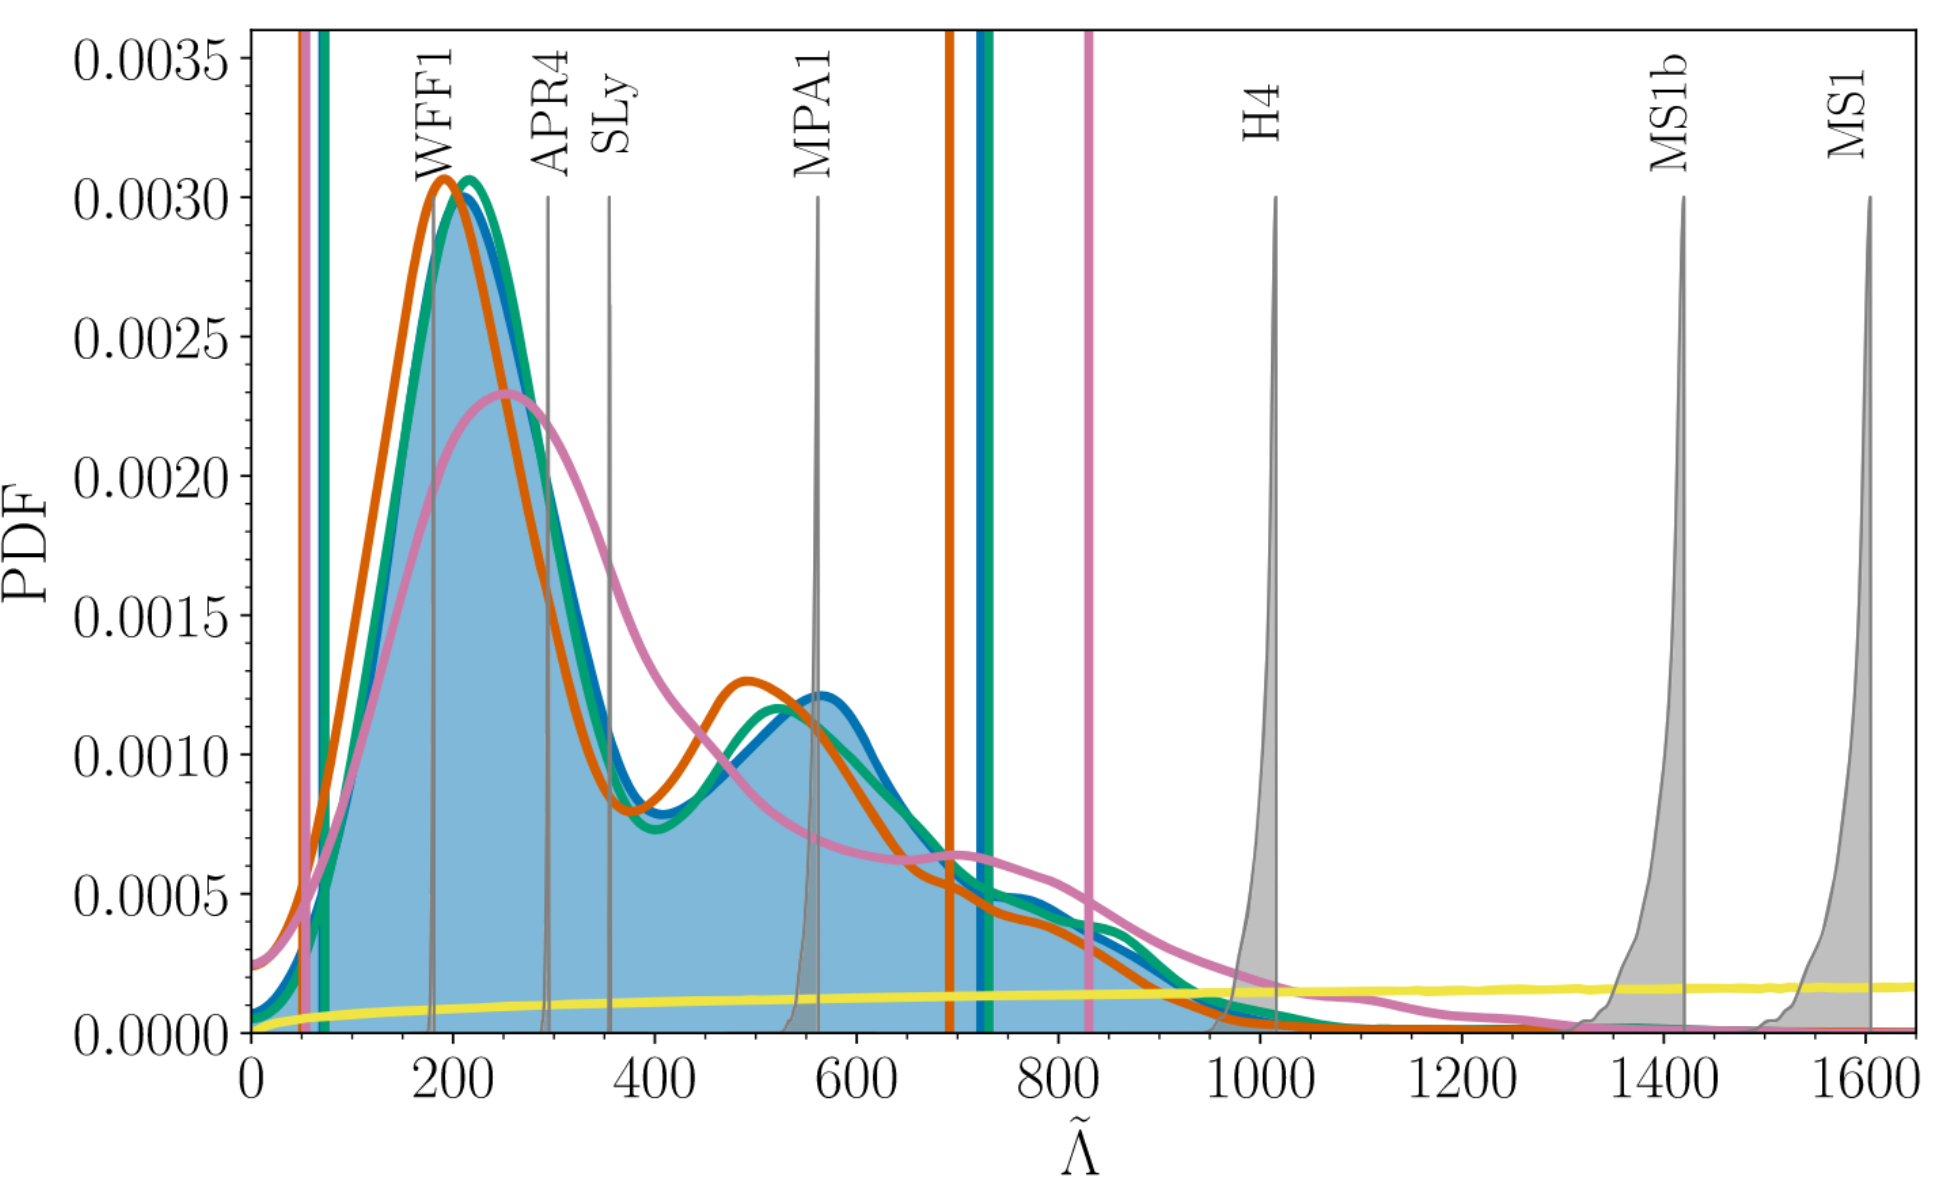
\includegraphics[width=0.65\textwidth]{Figures/GW170817_lambda_tilde.png}
    \end{figure}
  }
\end{frame}

\section{Future prospects}

\begin{frame}{Postmerger GW}

  \def\x{3mm}

  $\Lambda$ probes the inspiral, what about (post)merger?

  \quad $\rightarrow$ Need sensitive detectors~\cite{Maggiore:2019uih}!

  \begin{figure}[H]
    \centering
    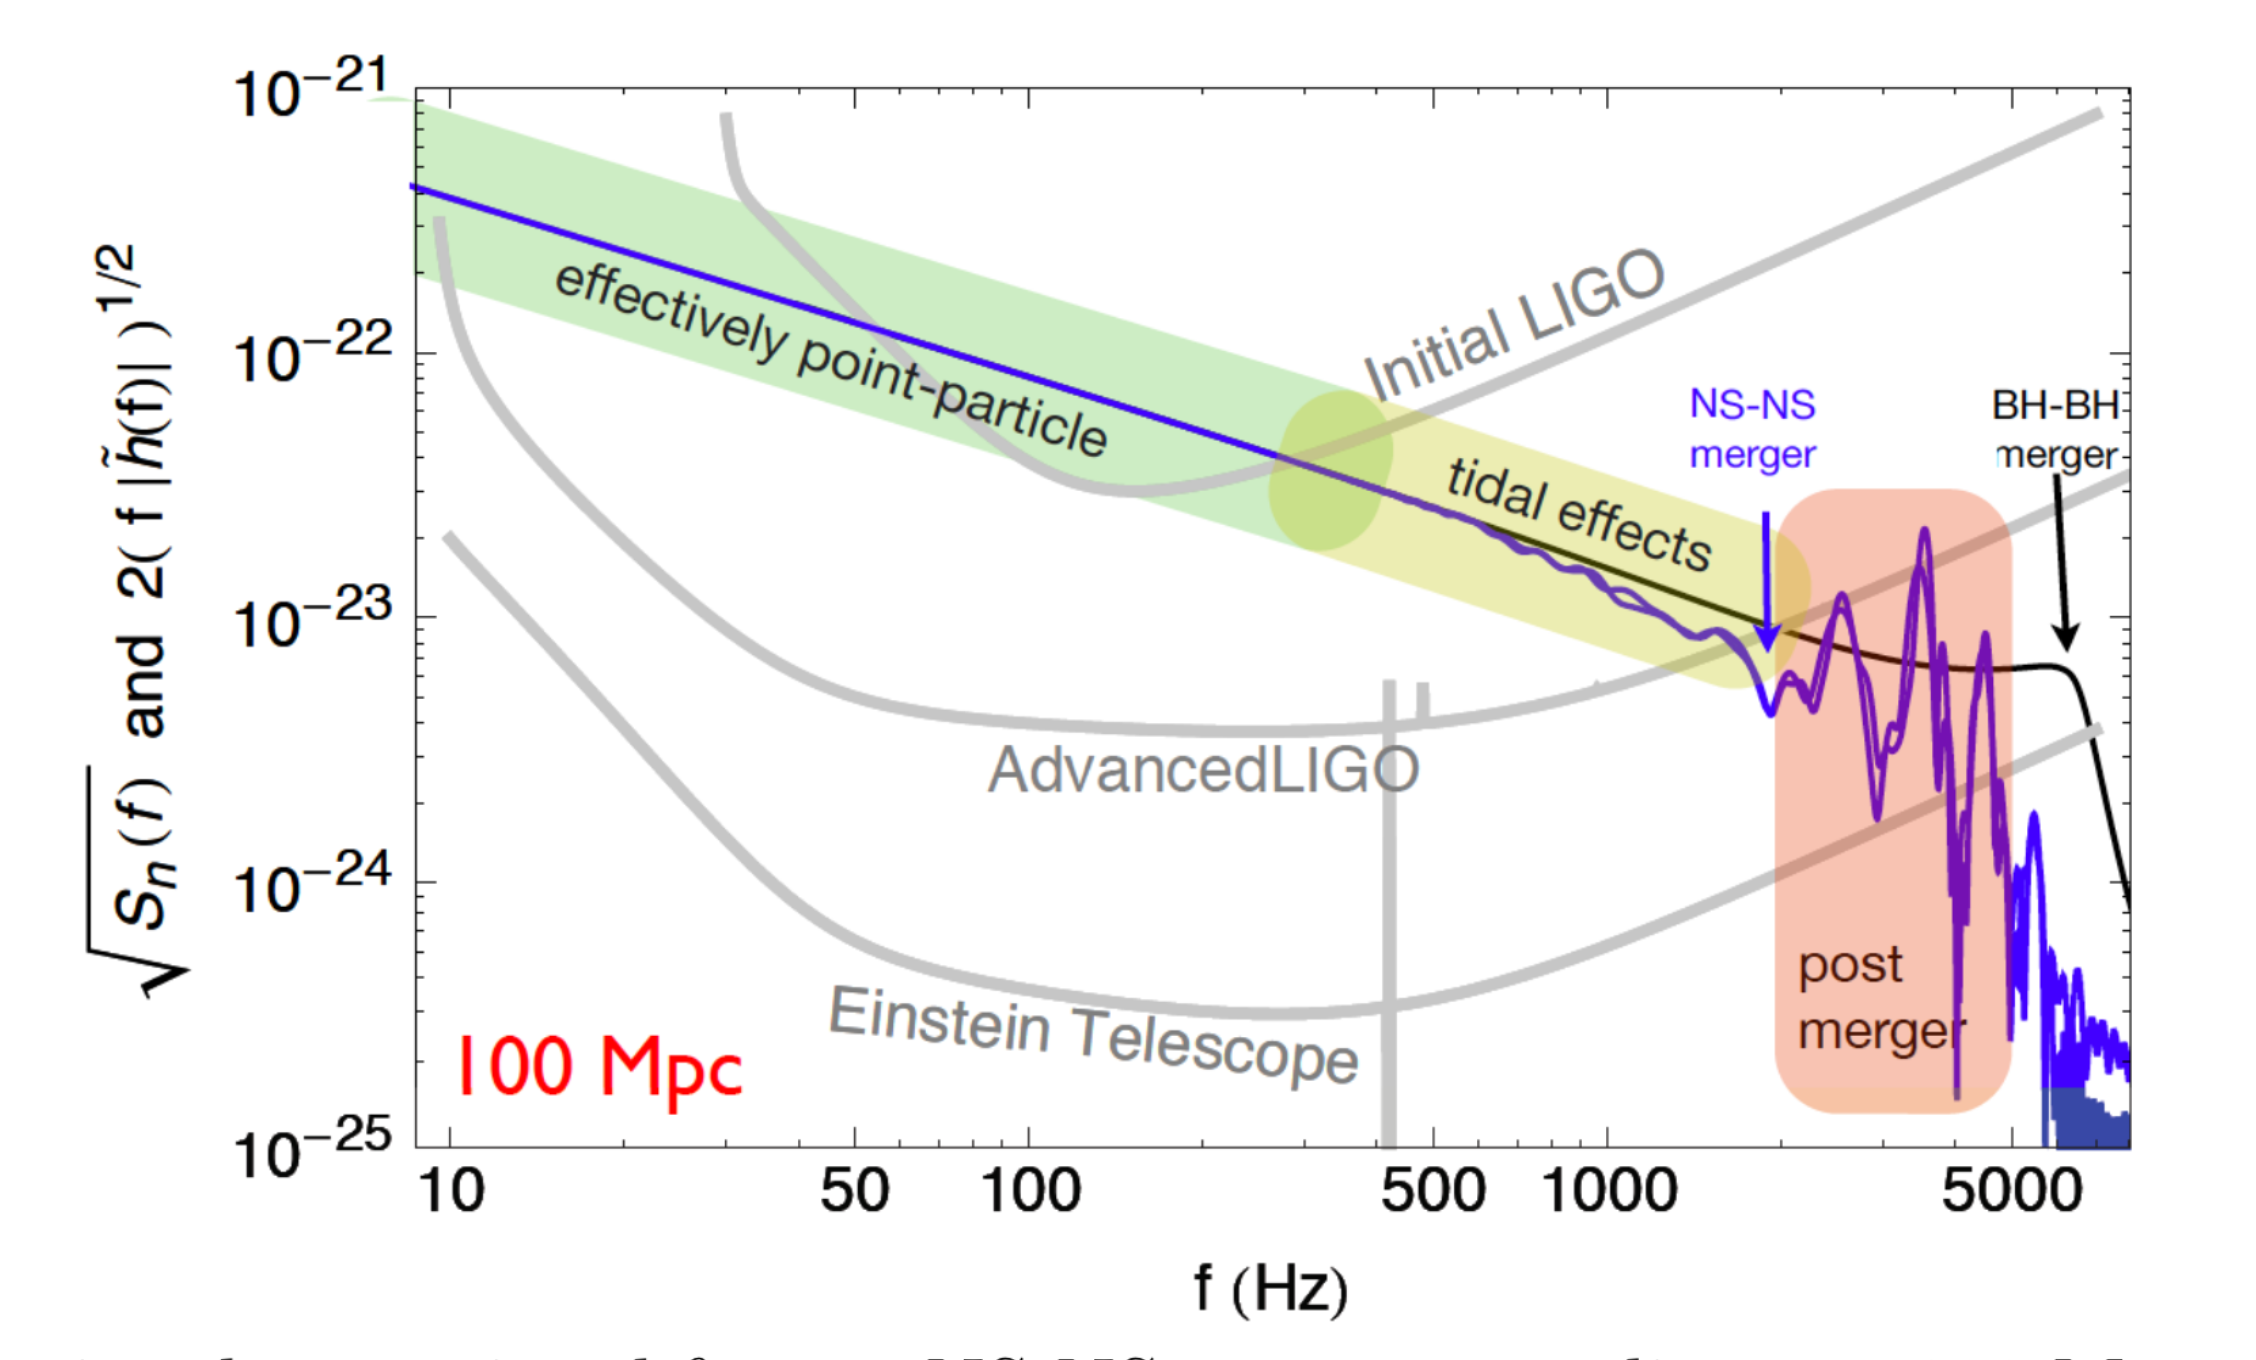
\includegraphics[width=0.85\textwidth]{Figures/PSD-and-postmerger.png}
  \end{figure}
\end{frame}

\begin{frame}{Challenges}

  \def\x{4mm}

  (Post)merger GW: needs expensive numerical relativity (NR) simulations, taking \red{temperature} into account!

  \vspace{\x}

  \begin{itemize}
    \item NR simulations: expensive, temperature is hard (?)
    
    \vspace{\x}

    \item Modelling GW signals: how to connect inspiral and (post)merger? Parameter estimation?
    
    \vspace{\x}
    
    \item Quasi-universal relations exist~\cite{Tsang:2019esi} -- can they be improved?
    
    \vspace{\x}
    
    \item ALICE at high temperature -- way to make connection?
  \end{itemize}

  \vspace{\x}

  Let us check out Ref.~\cite{Fields_2023} as an example. 
\end{frame}

\section{"Thermal Effects in Binary Neutron Star Mergers"}

\begin{frame}{"Thermal Effects in Binary Neutron Star Mergers"}

  \def\x{3mm}

  \begin{itemize}
    \item Isolated neutron star: $T = 0$ MeV (cold); merger: $T \sim 100$ MeV
    
    \vspace{\x}
    
    \item Ref.~\cite{Fields_2023}: \red{temperature effects} through modifying the specific heat capacity
    
    \vspace{\x}
    
    \item Perform parameter estimation with postmerger waveform from \cite{breschi2022kilohertz}
  \end{itemize}

  \only<1>{
    \begin{figure}
    \centering
    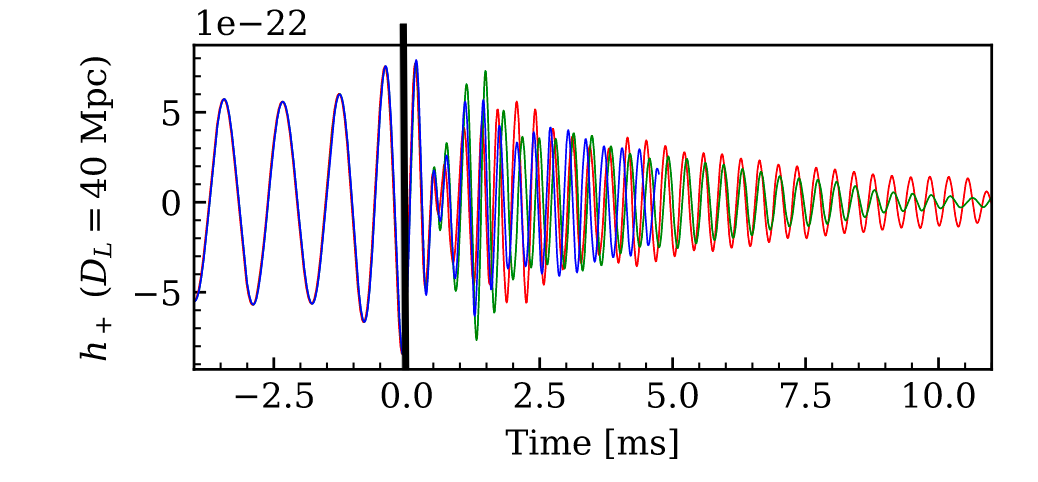
\includegraphics[width=0.75\textwidth]{Figures/postmerger_spectrum.png}
  \end{figure}
  }

  \only<2>{
    \begin{figure}
    \centering
    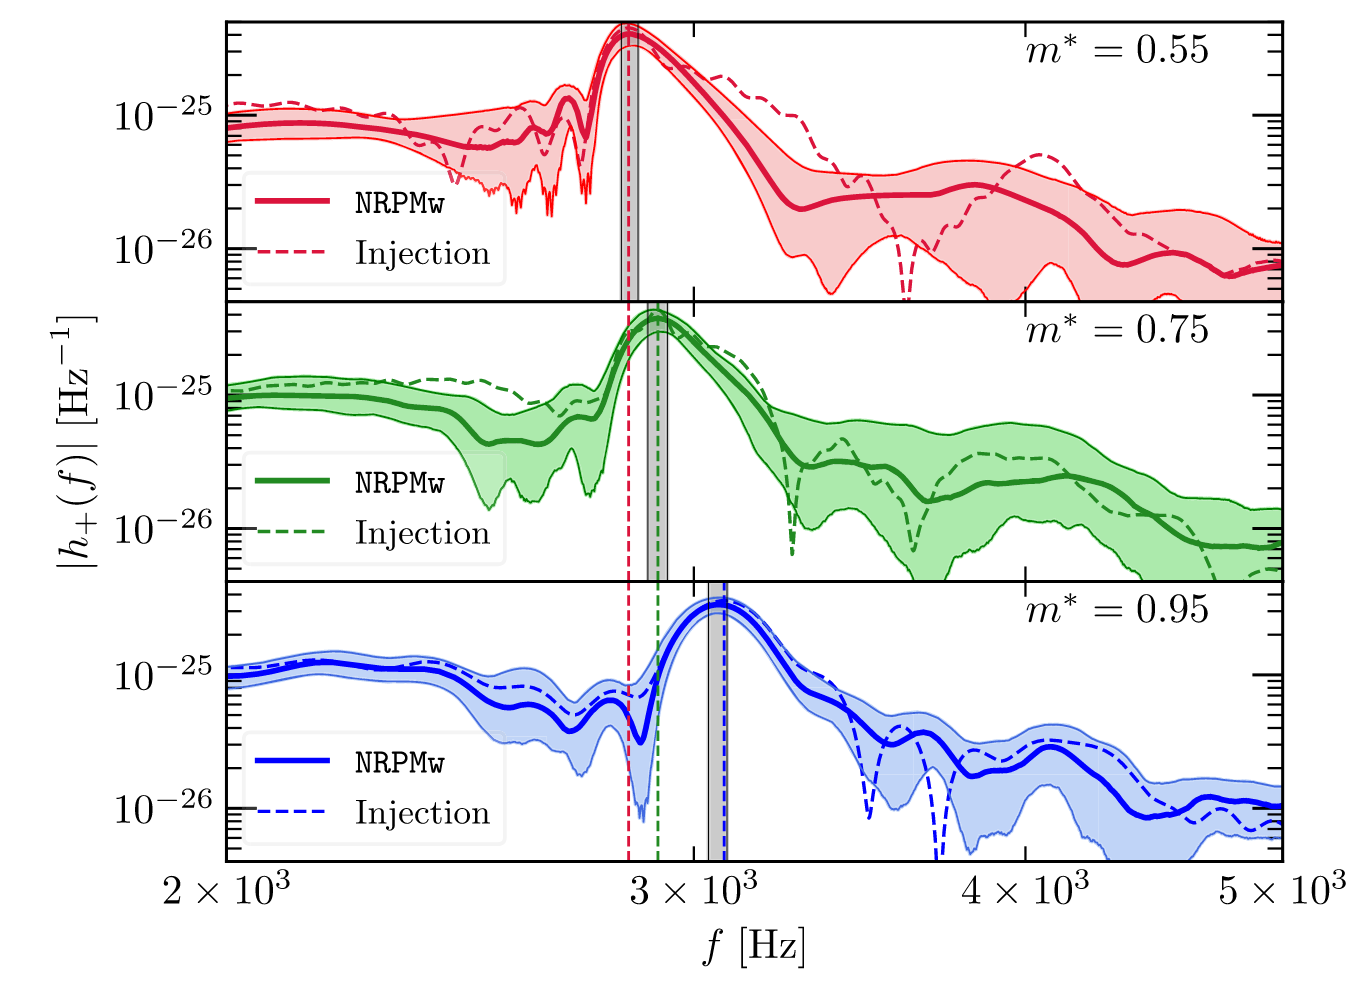
\includegraphics[width=0.6\textwidth]{Figures/postmerger_spectrum_varying_mstar.png}
  \end{figure}
  }

\end{frame}

\begin{frame}{Conclusions}

  \def\x{3mm}
  \begin{itemize}
    \item Inspiral of neutron stars: tidal deformability $\rightarrow$ cold EOS constraints
    
    \vspace{\x}
    
    \item Future GW detectors will measure postmerger spectrum
    
    \vspace{\x}
    
    \item Temperature effects have to be taken into account: challenges and opportunities
    
    \vspace{\x}
    
    \item Finite temperature might lead to a connection with ALICE
  \end{itemize}

  \begin{figure}
    \centering
    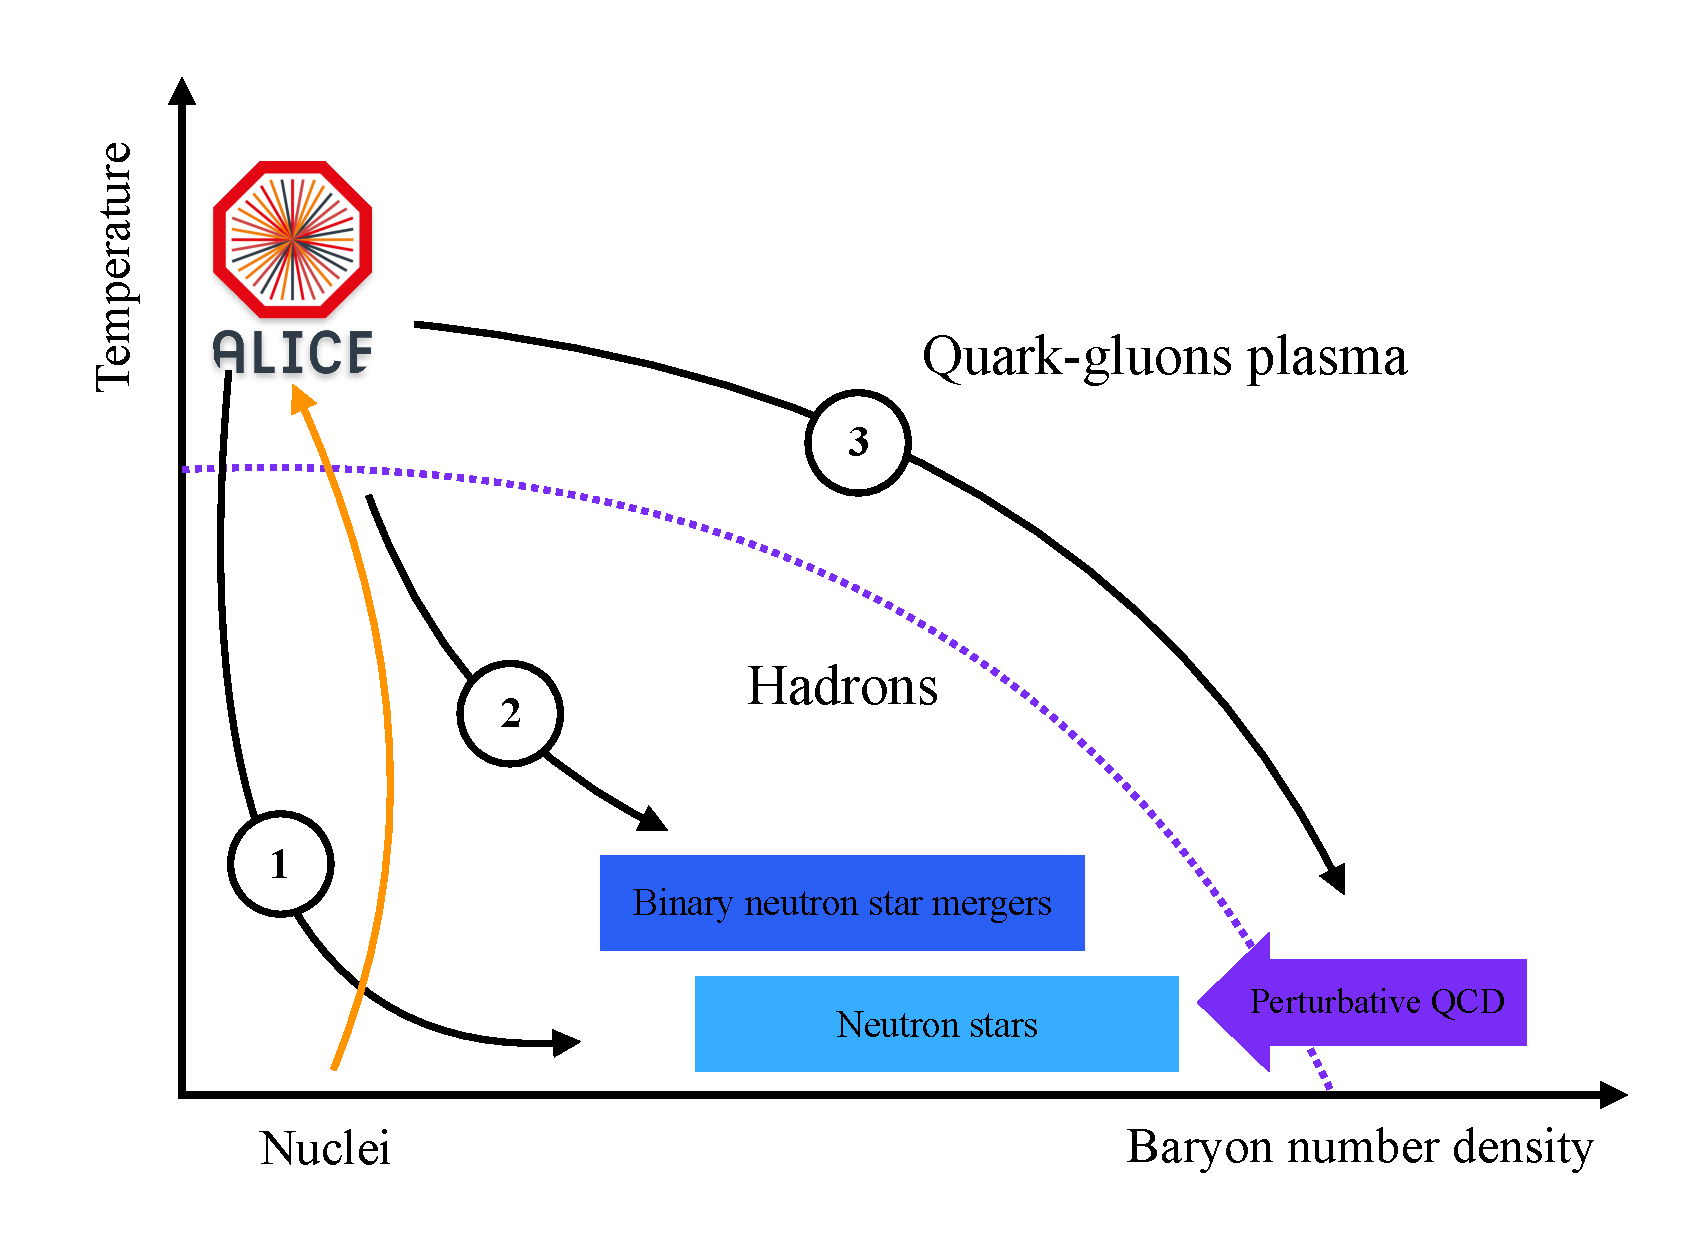
\includegraphics[width=0.5\textwidth]{Figures/QCD_phase_diagram.pdf}
  \end{figure}
  
\end{frame}


\begin{frame}{References}
  
    \printbibliography

\end{frame}

\end{document}

